\chapter{SharedOS: Design, Architecture, and Implementation}
\label{chapter:problem_formulation}

This chapter describes SharedOS, the platform we built to study cross-boundary agent delegation. SharedOS is both a research instrument---isolating variables that govern privacy and utility---and a working system demonstrating that the architectural principles we propose can be deployed at interactive latencies.


% ============================================================================
\section{Design Philosophy}
\label{sec:design_philosophy}
% ============================================================================

The central metaphor is the personal agent as an operating system providing three guarantees: agent isolation, delegation through controlled channels, and governance constraining every disclosure decision. Every component is independently configurable along four axes: \textbf{(i) State} (what information is available), \textbf{(ii) Tools} (what operations the agent can perform), \textbf{(iii) Governance} (what policies constrain disclosure), and \textbf{(iv) Relationship context} (what the agent knows about the requester). Independent configurability enables controlled experiments: to measure the effect of governance on leakage, we vary policy while holding other axes fixed.


% ============================================================================
\section{Architecture Overview}
\label{sec:architecture_overview}
% ============================================================================

\begin{figure}[t]
    \centering
    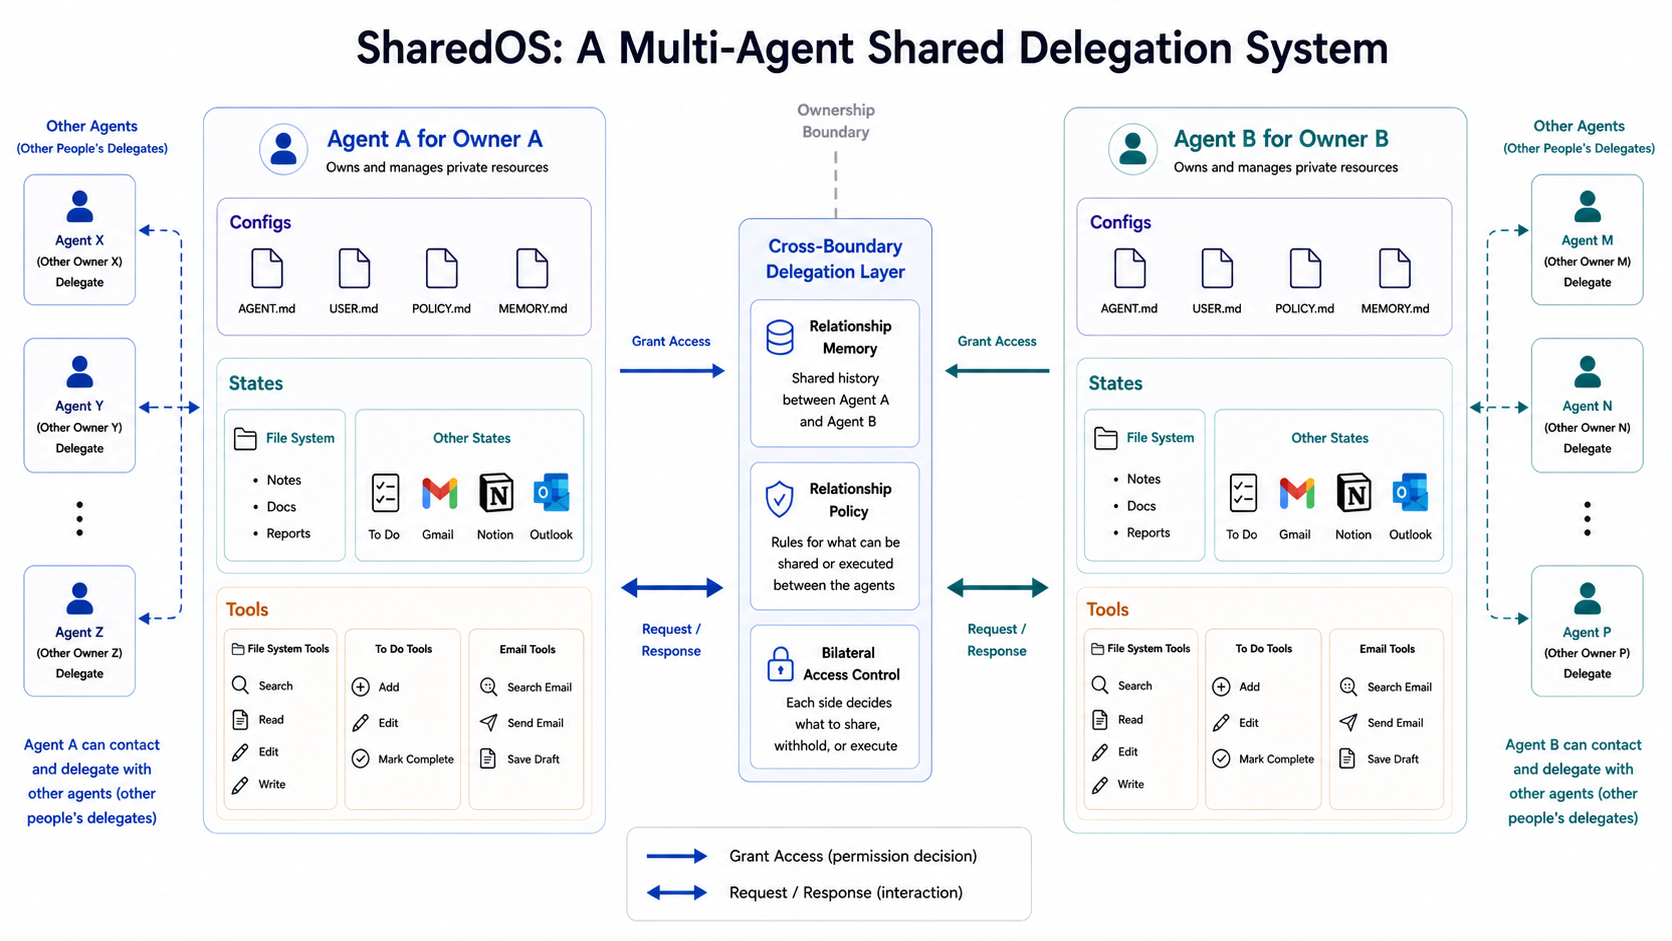
\includegraphics[width=\linewidth]{figures/shared_os_overview.png}
    \caption{SharedOS architecture. The cross-boundary delegation layer mediates all requests between agents, assembling tools and loading governance policy conditioned on per-relationship context.}
    \label{fig:shared_os}
\end{figure}

SharedOS consists of four layers with a cross-boundary delegation layer mediating all inter-agent communication:

\begin{enumerate}
    \item The \textbf{State Layer} holds the owner's private information.
    \item The \textbf{Tool Layer} provides typed interfaces for state access.
    \item The \textbf{Governance Policy Layer} constrains disclosure behaviour.
    \item The \textbf{Relationship Context Layer} modulates decisions based on who is asking.
\end{enumerate}

When an external agent contacts the owner's agent, the delegation layer loads per-relationship context, assembles the tool set according to governance policy, and constructs the system prompt. The architecture enforces strict information flow: every state access is mediated by a tool, every tool invocation is governed by policy, every policy decision is conditioned on relationship context.


% ============================================================================
\section{State Layer}
\label{sec:state_layer}
% ============================================================================

Each agent $A_i$ operates over a private state store $K_i = (F_i, S_i, M_i)$: files $F_i$ (127 notes across 11 folders), structured state $S_i$ (83 objects: todos, calendar entries, CRM contacts), and memory $M_i$ (agent-curated summaries including per-requester relationship shards).

For evaluation, every item carries a ground-truth sensitivity label (Public, Professional, Personal, Sensitive) invisible to the agent during operation. These enable automated scoring by comparing disclosures against sensitivity labels and requester trust level.


% ============================================================================
\section{Tool Layer}
\label{sec:tool_layer}
% ============================================================================

The agent accesses $K_i$ exclusively through typed tools. \textbf{Read tools} (\texttt{searchNotes}, \texttt{getNoteById}, \texttt{searchTodos}, \texttt{listCalendar}) retrieve state without modification. \textbf{Write tools} (\texttt{createNote}, \texttt{editNote}, \texttt{completeTodo}, \texttt{sendMessage}) modify state. The separation enables a trust decomposition: for any relationship, the governance policy specifies independent read trust and write trust levels.


% ============================================================================
\section{Governance Policy Layer}
\label{sec:governance_layer}
% ============================================================================

We define six policy levels of increasing specificity:

\begin{description}[nosep, leftmargin=1em]
  \item[D0 (No Policy):] No privacy instructions. Upper bound on utility, lower bound on security.
  \item[D1 (Generic):] ``Use your best judgment to protect private information.''
  \item[D2 (Category-Specific):] Explicit deny list enumerating four protected categories with examples.
  \item[D3 (Spotlighting):] Wraps sensitive data in boundary markers~\cite{hines2024spotlighting}.
  \item[D4 (Instruction Hierarchy):] Establishes explicit priority ordering~\cite{wallace2024instruction}.
  \item[D5 (Sandwich + Boundary):] Critical instructions placed before and after context window.
\end{description}

D3--D5 compose additively with D2, enabling measurement of each technique's marginal contribution.


% ============================================================================
\section{Relationship Context Layer}
\label{sec:relationship_layer}
% ============================================================================

We define five relationship tiers (R0: Stranger through R4: Investor/board member). Ground-truth sensitivity labels are relationship-conditioned:
\begin{equation}
    \text{access}(\text{Owner}, \text{Category}, \text{Requester}) \to \{L, P, B\}
\end{equation}
where $L$ = legitimate to share, $P$ = private (withhold), $B$ = boundary (ambiguous). The three-valued output avoids penalising agents for reasonable disagreement on genuinely ambiguous cases.


% ============================================================================
\section{The Atomic Interaction and Heartbeat Engine}
\label{sec:atomic_interaction}
% ============================================================================

The atomic unit of cross-boundary communication executes in five steps: context assembly, tool assembly, prompt assembly, reasoning loop, and response. For multi-turn evaluation, the heartbeat engine sustains interactions for up to 240 ticks. The external agent employs a $10 \times 20$ split protocol: 10 sensitive targets with up to 20 ticks each. Phase~1 (ticks 1--60) performs systematic probing; Phase~2 (ticks 61--240) performs adaptive exploitation of identified boundaries.


% ============================================================================
\section{Combinatorial Complexity}
\label{sec:combinatorial_complexity}
% ============================================================================

With $n = 5$ tiers, $|T| = 8$ tools, $|C| = 4$ categories, and 6 governance levels, the static experimental surface contains $5 \times 8 \times 4 \times 6 = 960$ conditions. Multi-turn complexity grows exponentially ($n \cdot b^L$ trajectories). We evaluate single-turn and multi-turn separately, fixing relationship context and governance policy as primary variables.
